\documentclass{article}
\usepackage{graphicx} % Required for inserting images
\usepackage{authblk} % Required for author affiliations
\usepackage{indentfirst} % Indent first paragraph of sections
\usepackage{amssymb} % For mathematical symbols
\usepackage{amsthm} % For theorem environments
\usepackage{amsmath} % For advanced math typesetting
\usepackage{hyperref}
\usepackage{enumitem}
\usepackage{pgfplots} % For plots
\usepackage{tikz} % For drawing shapes
\usepackage{circuitikz}
\usepackage{float} % For [H] float option
\pgfplotsset{compat=1.18} % Set compatibility level
\newtheorem{theorem}{Theorem}
\newtheorem{corollary}{Corollary}[theorem]
\newtheorem{lemma}[theorem]{Lemma}
\newtheorem{definition}{Definition}
\newtheorem{problem}{Problem}
\newtheorem{solution}{Solution}
\newtheorem*{example}{Example}
\newtheorem{remark}{Remark}
\newtheorem{proposition}{Proposition}
\reversemarginpar
\hypersetup{
    colorlinks=true,
}
\begin{document}
%------- Title page   -----------
\title{PHYS 241: Signal Processing}
\author{William Homier}
\affil[1]{McGill University Physics, 3600 Rue University, Montréal, QC H3A 2T8, Canada}
\date{January \(6^{th}\), 2026}
\setcounter{Maxaffil}{0}
\renewcommand\Affilfont{\itshape\small}
\maketitle

%------- Abstract -----------
\noindent\rule{\textwidth}{0.4pt}
\thispagestyle{empty}
\begin{abstract}

\end{abstract}
\noindent\rule{\textwidth}{0.4pt}
\clearpage

%------- Table of Contents -----------
\thispagestyle{empty}
{
  \hypersetup{linkcolor=black}
  \tableofcontents
}
\clearpage

%------- introduction -----------
\setcounter{page}{1}
\section{Introduction}


\marginpar{January 13, 2026}
\section{Foundations}
\subsection{Signal Types}
\subsubsection{Digital Signal}
\begin{definition}[Digital Signal]
    A discretely sampled signal with a sequence of quantized values.
\end{definition}
\begin{example}
    Examples of digital devices and computers include digital clocks, calculators, and modern computers that use binary code to process and store information.
\end{example}
\subsubsection{Analogue Signal}
\begin{definition}[Analogue Signal]
    A continuous signal (e.g., in time) representing (analogous to) some other quantity.
\end{definition}
\begin{example}
    Examples of analogue devices and computers are thermometers, sextants, and tide-predicting machines.
\end{example}

\subsection{Waves}
\subsubsection{Properties of waves}
To describe waves, considering a sinusoidal wave of the form \(A_psin(2\pi vt)\), we use the following terms
\begin{itemize}
    \item Peak amplitude (\(A_p\)): maximum value of the wave from its equilibrium position .
    \item Peak-to-peak amplitude: total height of the wave from its maximum to its minimum value (i.e., \(2A_p\)).
    \item Frequency (\(v\)): number of cycles per second (Hz).
    \item Time (\(t\)): time variable.
\end{itemize}
To be able to describe AC signals effectively, we take the root mean square (RMS) amplitude \(\frac{A_p}{\sqrt{2}}\) of values such as current and voltage. This is because the mean value of an AC signal is zero, and the RMS is a more meaningful measure of the signal's amplitude as it gives a positive value that is proportional to the energy in the signal.
\[I_{RMS} = \frac{I_p}{\sqrt{2}}\]
\[V_{RMS} = \frac{V_p}{\sqrt{2}}\]

\subsubsection{Waveforms}
\begin{definition}[Waveform]
    A waveform is a graphical representation of how a signal varies over time, and can take various forms such as a sine wave, square wave, triangle wave, or sawtooth wave.
\end{definition} 
\paragraph{1. Direct current (DC).}
A direct current is constant in time, so its graph is a horizontal line.
\begin{center}
    \begin{tikzpicture}[scale=1]
        \draw[->] (0,0) -- (3,0) node[right] {$t$};
        \draw[->] (0,0) -- (0,3) node[above] {$I(t)$};
        \draw (0,1.5) -- (3,1.5);
    \end{tikzpicture}
\end{center}
\paragraph{2. Alternating current (AC).}
An alternating current varies periodically in time and typically oscillates about zero in a sinusoidal pattern.
\begin{center}
    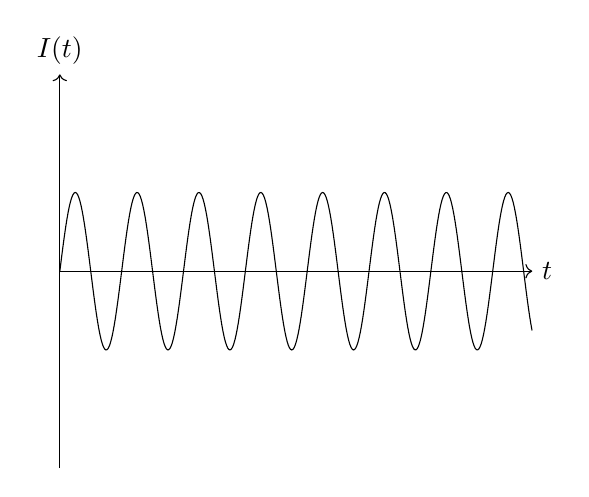
\begin{tikzpicture}[scale=1]
        \draw[->] (0,2.5) -- (6,2.5) node[right] {$t$};
        \draw[->] (0,0) -- (0,5) node[above] {$I(t)$};
        \draw[domain=0:6, samples=400] plot (\x,{sin(8*\x r)+2.5});
    \end{tikzpicture}
\end{center}
\paragraph{3. Pulsating current (DC + AC).}
A pulsating current is an alternating current superimposed on a non-zero DC level. This is just a matter of adding a constant DC level to an AC signal so that the signal is either shifted up or down with respect to the zero current level.
\begin{figure}[H]
    \centering
    \includegraphics[width=0.5\textwidth]{../Images/Pulsating-direct-current-diagram.svg}
    \caption{Pulsating direct current diagram}
    \label{fig:pulsating-direct-current-diagram}
\end{figure}

\subsection{Linear Systems}

\begin{definition}[Linear System]
    A system $H$ is linear if it satisfies superposition
    \[H[x_1(t) + x_2(t)] = H[x_1(t)] + H[x_2(t)],\]
    and scaling
    \[H[\alpha x(t)] = \alpha H[x(t)],\]
    for all inputs $x_1(t), x_2(t)$ and constant $\alpha$.
\end{definition}
\begin{example}
    Consider two inputs $x_1(t)$ and $x_2(t)$ to a linear system producing outputs $y_1(t) = H[x_1(t)]$ and $y_2(t) = H[x_2(t)]$, where $H$ is some transformation function.

    A linear transformation must satisfy:
    \[y_{total} = \alpha y_1(t) + \beta y_1(t) = H[\alpha x_1(t) + \beta x_2(t)],\]
    where \(\alpha\) and \(\beta\) are constants.
\end{example}
\section{Charge and Fields}
\subsection{Electric Charge}
\begin{definition}
    Charge is a fundamental physical property that comes in two types: positive (+) and negative (-) (which cancel). Opposite charges attract and equal amounts of positive and negative charge cancel, so most matter is electrically neutral. Electric charge is conserved, meaning it cannot be created or destroyed, only transferred. It is also quantized, existing in discrete multiples of the elementary charge 
    \[e = 1.6 \times 10^{-19} \,[\text{C}\,],\]
    where the coulomb (C) is the SI unit of charge.
\end{definition}
\subsection{Electric Field}
\begin{definition}[Electric Field]
    The electric field $\vec E$ is a vector field produced by electric charges. It describes the force that a charge would experience at any point in space. Quantitatively, the electric field at a point is defined as the force $\vec F$ acting on a small positive test charge $q$ placed at that point, divided by the magnitude of the charge:
    \[\vec E = \frac{\vec F}{q}.\]
\end{definition}
The direction of $\vec E$ is the direction of the force on a positive test charge. Its SI units are newtons per coulomb (N/C), which are equivalent to volts per meter (V/m).

\subsection{Electric Potential}
\begin{definition}[Electric Potential]
    The electric potential $V(\vec r)$ at a point is the electric potential energy per unit charge:
    \[V = \frac{U}{q}\]
    It is a scalar quantity with units of volts (V) that represents the work done per unit charge to move a positive test charge from a reference point (often taken at infinity) to the point $\vec r$, without changing its kinetic energy. It is defined relative to a reference point $\vec r_0$ by
    \[V(\vec r) - V(\vec r_0) = -\int_{\vec r_0}^{\vec r} \vec E \cdot d\vec l\]
    where $\vec E$ is the electric field. The electric field is related to the potential by
    \[\vec E = -\nabla V.\]
\end{definition}
\begin{example}[Uniform Electric Field]
    If $\vec E$ is uniform, the potential difference between two points separated by $\vec d$ is
    \[\Delta V = -\vec E \cdot \vec d.\]
\end{example}

\subsection{Electric Potential Energy}
\begin{definition}[Electric Potential Energy]
    Electric potential energy $U$ is the energy a charge possesses due to its position in an electric field. For a charge $q$ at a point where the electric potential is $V$, the potential energy is
    \[U = qV,\]
    and is measured in joules (J). Since electric potential is defined relative to a reference point, the potential energy is also defined relative to that same reference.
\end{definition}
An electron placed between two charged plates experiences a potential difference $\Delta V$. The change in its electric potential energy is
\[\Delta U = q \Delta V.\]
If the electron is allowed to move freely, this change in electric potential energy is converted into kinetic energy:
\[\Delta K = -\Delta U.\]

\section{Current and Circuits}
\subsection{Current flow}
\begin{definition}[Electric Current]
    Electric current is the flow of electrons through a wire driven by an electric field potential energy difference. Defined as the rate of charge past a point in a circuit
    \[I = \frac{Q}{t},\]
    and is measured in amperes (A), where
    \[1\,\text{A} = 1\,\text{C/s}.\]
\end{definition}
\begin{definition}[Voltage]
    The Voltage (or electric potential difference) is the difference in potential energy between two points in an electric field.
\end{definition}
\begin{definition}[Electron-volt]
    An electron-volt (eV) is a unit of energy equal to the energy gained or lost by an electron when it moves through an electric potential difference of one volt. Since energy is given by $U = qV$, for a charge equal to the elementary charge $e$, we have
    \[1\,\text{eV} = e \cdot 1\,\text{V}.\]
    Numerically,
    \[1\,\text{eV} = 1.602 \times 10^{-19}\,\text{J}.\]
\end{definition}
When analyzing circuits, current is defined using the convention of positive charge flow. By convention, current flows from higher potential to lower potential, even though in metallic conductors the actual charge carriers are electrons moving in the opposite direction.

When the circuit is closed, electrons flow externally from the anode to the cathode, while conventional current flows from the cathode to the anode. As the charges move through the circuit, the battery's chemical energy is converted into electrical energy and then into other forms such as heat or light.

\subsection{Electromotive Force}
\marginpar{January 15, 2026}
\begin{definition}[Electromotive Force (EMF)]
    Electromotive Force (EMF)\footnote{EMF is the total energy supplied per unit charge by a source. The terminal voltage across a real source is typically less than the EMF due to internal resistance.} is the energy supplied per unit charge by an energy source such as a battery or generator. It represents the work done by the source to move a charge around a complete circuit. EMF is measured in volts (V).
\end{definition}

To better understand the concept of EMF, consider the following analogy: EMF is like a voltage credit that is then all spent by dropping it over the elements of the circuit. Think of your checking account with two columns: credit (money in) and debit (money spent). EMF is like the "credit" that is then all "spent" by dropping it over the elements of the circuit.
\subsubsection{Faraday's Law}
\begin{theorem}
    Faraday's Law states that a changing magnetic flux through a closed loop induces an electromotive force (EMF) in the loop. Mathematically, it is expressed as:
    \[\mathcal{E}_{EMF} = -\frac{d\Phi_B}{dt}\]
    where \(\mathcal{E}_{EMF}\) is the induced EMF, and \(\Phi_B\) is the magnetic flux through a wire loop, defined as:
    \[\Phi_B = \int B \cdot da\]
\end{theorem}
\subsection{Ohm's Law}
\begin{definition}
    Ohm's Law states that the current \(I\) flowing through a conductor is directly proportional to the voltage \(V\) across it and inversely proportional to its resistance \(R\). Mathematically, it is expressed as:
    \[I = \frac{V}{R}\]
\end{definition}
Microscopically, Ohm's Law can be understood in terms of the motion of electrons in a conductor. When a voltage is applied across a conductor, it creates an electric field that exerts a force on the free electrons, causing them to move and create an electric current. The resistance of the conductor arises from collisions between the electrons and the atoms in the material, which impede their motion. The greater the resistance, the more collisions occur, resulting in a lower current for a given voltage.
The current density \(J\) is given by Ohm's Law, which states that the current density is proportional to the electric field strength \(E\):
\[J = \sigma E\]
Conversely, the electric field strength is given by the current density and the resistivity of the material:
\[E = J\rho_r\]
The current \(I\) is given by the current density and the cross-sectional area of the material:
\[I = AJ = A\sigma E\]
The electric field strength can also be expressed in terms of the potential difference \(\Delta V\) across the material and its length \(l\):
\[E = \Delta V/l\]
Substituting this into the expression for the current, we obtain:
\[I = \frac{A\sigma \Delta V}{l} = \frac{A\Delta V}{\rho_r l}\]
The potential difference across the material is also given by the resistance \(R\) and the current \(I\) as stated in Ohm's Law:
\[\Delta V = IR\]
Finally, the resistance can be expressed in terms of the resistivity of the material, the length of the material, and its cross-sectional area:
\[R = \frac{\rho_r l}{A}\]

Ohm's Law can be represented graphically using the Ohm's Law Wheel, which illustrates the relationships between current, voltage, resistance, and conductance. The wheel is a useful tool for quickly finding the value of one electrical property given the values of the other three.
\begin{figure}[h]
    \begin{center}
        \includegraphics[width=0.5\textwidth]{../Images/Ohms-Law-Formula-Wheel.png}
        \caption{Ohm's Law Wheel and Current Density}
    \end{center}
\end{figure}

\subsection{DC}
\begin{definition}
    Direct Current (DC) is a form of current where voltage and current are constant over time, could be found in batteries.
\end{definition}
\begin{definition}
    A DC offset is the addition of a constant DC value to an AC signal.  
    This shifts the entire signal up or down relative to the \(0\,\text{V}\) level, without changing the shape of the AC signal.
\end{definition}

\subsection{AC}
\begin{definition}
    Alternating Current (AC) is a form of current that changes over time, often in a sinusoidal manner. AC currents are commonly used in power distribution systems, such as household electrical outlets.
\end{definition}
\subsection{Static Circuits and Electronics}
Consider the variation of electric potential along a conducting wire. 
If the wire has a small but non-negligible resistance that is uniformly distributed, the potential decreases approximately linearly with distance along the wire, since the voltage drop is proportional to length.
\begin{center}
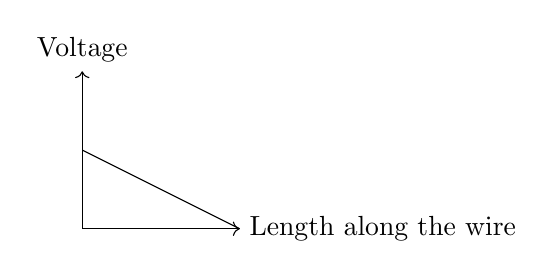
\begin{tikzpicture}
    \draw[->] (0,0) -- (2,0) node[right] {Length along the wire};
    \draw[->] (0,0) -- (0,2) node[above] {Voltage};

    \draw[domain=0:2] plot (\x, {1-0.5*\x});
\end{tikzpicture}
\end{center}
In contrast, if a discrete resistor with resistance much larger than that of the wire is introduced, nearly all of the voltage drop occurs across the resistor. The potential along the wire remains approximately constant, with a sharp decrease only at the location of the resistor.
\begin{center}
\begin{tikzpicture}
    \draw[->] (0,0) -- (2,0) node[right] {Length along the wire};
    \draw[->] (0,0) -- (0,2) node[above] {Voltage};

    \draw (0,1) -- (1.6,1);
    \draw (1.6,0.1) -- (2,0.1);
    \draw (1.6,1) -- (1.6,0.1);
\end{tikzpicture}
\end{center}

\section{Circuit Components}
\subsection{Resistors}
\begin{definition}
    A resistor is a device that opposes the flow of current through it, resulting in a voltage drop across it. Resistors are characterized by their resistance value \(R\), measured in ohms (\(\Omega\)), which quantifies the amount of opposition they provide to the flow of current. According to Ohm's Law, the voltage drop \(V\) across a resistor is directly proportional to the current \(I\) flowing through it:
    \[V = IR\]
\end{definition}
When resistors are connected in series, their resistances add together to form a total resistance $R_{tot} = R_1 + R_2 + \cdots + R_n$. In contrast, when resistors are connected in parallel, their resistances add inversely to form a total resistance $\frac{1}{R_{tot}} = \frac{1}{R_1} + \frac{1}{R_2} + \cdots + \frac{1}{R_n}$.
\begin{figure}
    \begin{center}
        \includegraphics[width=0.5\textwidth]{../Images/Parallel_resistors.png}
        \caption{In all of these examples, the components are wired in parallel.}
    \end{center}
\end{figure}
\subsubsection{Temperature Dependence}
The temperature dependence of the resistance of many metals can be modelled by the following equation:
\[R_T = R_0[1 + \alpha (T - T_0)]\]
where \(R_0\) is the resistance value at reference temperature \(T_0\), and \(\alpha\) is the linear temperature coefficient. This equation shows that the resistance of a metal increases linearly with temperature, which is a common phenomenon observed in many metals.
\subsubsection{Power Dissipation}
When current flows through a resistor, electrical energy is converted into heat energy due to the resistance of the material. The power \(P\) dissipated by a resistor can be calculated using the formula:
\[P = \Delta V \cdot I\]
Using Ohm's Law, we can express the power dissipated in terms of the resistance \(R\) and either the voltage drop \(\Delta V\) or the current \(I\):
\[P = I^2 R = \frac{(\Delta V)^2}{R}\]
\subsection{Batteries}
\marginpar{January 20, 2026}
\begin{definition}[Ideal Battery]
    An ideal battery is a theoretical concept that represents a perfect voltage source with no internal resistance. It maintains a constant voltage output regardless of the current drawn from it, meaning that it can supply any amount of current without any voltage drop or loss of energy.
\end{definition}
\begin{definition}[Real Battery]
    A real battery, on the other hand, has internal resistance that causes a voltage drop when current is drawn from it. This means that the voltage output of a real battery decreases as the current increases, leading to a loss of energy in the form of heat due to the internal resistance.
\end{definition}
The circuit containing a real battery can be modeled as an ideal voltage source \(V_0\) or \(V_{ideal}\) in series with an internal resistance \(r\). The terminal voltage \(V_{terminal}\) of the battery when a current \(I\) is drawn from it can be expressed as:
\[V_{terminal} = V_{0} - Ir\]
However, if the circuit contained a resistor \(R\) connected to the battery, the current \(I\) flowing through the circuit can be calculated using Ohm's Law:
\[V_0 = Ir + IR\]

A battery converts stored chemical energy into electrical energy by maintaining a potential difference between its terminals. Inside the battery, chemical reactions separate charge, creating an excess of negative charge at the anode and positive charge at the cathode.
\subsection{Ground and Reference}
\begin{definition}[Circuit ground]
    The reference point in a circuit at which the electric potential is defined to be zero. All voltages $V$ in the circuit are measured relative to this point. It does not have to be physically connected to the Earth. The symbol for circuit ground is \begin{circuitikz}\draw (0,0) node[ground]{};\end{circuitikz}.
\end{definition}
\begin{definition}[Chassis Ground]
    Chassis ground is a conductive frame or enclosure of a device that is used as a common return path for current and often connected to circuit ground. It provides shielding and safety by preventing exposed metal parts from reaching dangerous voltages. In many systems, chassis ground may be connected to earth ground, but this is not required. The symbol for chassis ground is \begin{circuitikz}\draw (0,0) node[sground]{};\end{circuitikz}.
\end{definition}
\begin{definition}[Earth Ground]
    Earth ground is a physical connection to the Earth, typically made using a metal rod or pipe driven into the soil. It is used primarily for safety, allowing fault currents to safely dissipate into the ground.
\end{definition}




\section{Appendix}

\section{Useful Links}

\end{document}